\documentclass[12pt]{article}
\title{INFO-F-403: Project Super-Fortran Part 1 Lexer analyser}
\author{Sefu Kevin and Abou Zaidi Ahmed}
\usepackage{textcomp}
\usepackage{graphicx}
\usepackage{float}
\begin{document}
\maketitle
\section{Introduction}
In this project we were requested to design and write a compiler for Super-Fortran. It is a very simple 
imperative language. The project is divided in 3 parts and for this second part we had to produce 
the parser of the compiler. The parser is the tools that perform the syntax analysis of a sequences of tokens and verify if
those tokens are conform to the rules of grammar. During the parsing, the parse had to build the derivation tree.

There exist severals methods of building a parser. In our case we choose to design a recursive decent ll(1) parser.

\section{Grammar}
We did not find any useless rule. They all are accessible and productive.
\begin{description}
\item[\textbf{[1]}]{ \textbf{\textlangle{}Program\textrangle{}}  $\rightarrow$ BEGINPROG \textbf{[ProgName]} \textbf{[EndLine]} \textbf{\textlangle{}Variables\textrangle{}}  \textbf{\textlangle{}Code\textrangle{}}  ENDPROG}
\item[\textbf{[2]}]{ \textbf{\textlangle{}Variables\textrangle{}}  $\rightarrow$ VARIABLES \textbf{\textlangle{}VarList\textrangle{}}  \textbf{[EndLine]}}
\item[\textbf{[3]}]{ \textbf{\textlangle{}Variables\textrangle{}}  $\rightarrow \varepsilon$}
\item[\textbf{[4]}]{ \textbf{\textlangle{}VarList\textrangle{}}  $\rightarrow$ \textbf{[VarName]} \textbf{\textlangle{}VarList\_prim\textrangle{}} }
\item[\textbf{[5]}]{ \textbf{\textlangle{}VarList\_prim\textrangle{}}  $\rightarrow$ , \textbf{[VarName]} \textbf{\textlangle{}VarList\_prim\textrangle{}} }
\item[\textbf{[6]}]{ \textbf{\textlangle{}VarList\_prim\textrangle{}}  $\rightarrow \varepsilon$}
\item[\textbf{[7]}]{ \textbf{\textlangle{}Code\textrangle{}}  $\rightarrow$ \textbf{\textlangle{}Instruction\textrangle{}}  \textbf{[EndLine]} \textbf{\textlangle{}Code\textrangle{}} }
\item[\textbf{[8]}]{ \textbf{\textlangle{}Code\textrangle{}}  $\rightarrow \varepsilon$}
\item[\textbf{[9]}]{ \textbf{\textlangle{}Instruction\textrangle{}}  $\rightarrow$ \textbf{\textlangle{}Assign\textrangle{}} }
\item[\textbf{[10]}]{ \textbf{\textlangle{}Instruction\textrangle{}}  $\rightarrow$ \textbf{\textlangle{}If\textrangle{}} }
\item[\textbf{[11]}]{ \textbf{\textlangle{}Instruction\textrangle{}}  $\rightarrow$ \textbf{\textlangle{}While\textrangle{}} }
\item[\textbf{[12]}]{ \textbf{\textlangle{}Instruction\textrangle{}}  $\rightarrow$ \textbf{\textlangle{}For\textrangle{}} }
\item[\textbf{[13]}]{ \textbf{\textlangle{}Instruction\textrangle{}}  $\rightarrow$ \textbf{\textlangle{}Print\textrangle{}} }
\item[\textbf{[14]}]{ \textbf{\textlangle{}Instruction\textrangle{}}  $\rightarrow$ \textbf{\textlangle{}Read\textrangle{}} }
\item[\textbf{[15]}]{ \textbf{\textlangle{}Assign\textrangle{}}  $\rightarrow$ \textbf{[VarName]} := \textbf{\textlangle{}ExprArith\textrangle{}} }
\item[\textbf{[16]}]{ \textbf{\textlangle{}ExprArith\textrangle{}}  $\rightarrow$ \textbf{\textlangle{}Term\textrangle{}}  \textbf{\textlangle{}ExprArith\_prim\textrangle{}} }
\item[\textbf{[17]}]{ \textbf{\textlangle{}ExprArith\_prim\textrangle{}}  $\rightarrow$ + \textbf{\textlangle{}Term\textrangle{}}  \textbf{\textlangle{}ExprArith\_prim\textrangle{}} }
\item[\textbf{[18]}]{ \textbf{\textlangle{}ExprArith\_prim\textrangle{}}  $\rightarrow$ - \textbf{\textlangle{}Term\textrangle{}}  \textbf{\textlangle{}ExprArith\_prim\textrangle{}} }
\item[\textbf{[19]}]{ \textbf{\textlangle{}ExprArith\_prim\textrangle{}}  $\rightarrow \varepsilon$}
\item[\textbf{[20]}]{ \textbf{\textlangle{}Term\textrangle{}}  $\rightarrow$ \textbf{\textlangle{}Atom\textrangle{}}  \textbf{\textlangle{}Term\_prim\textrangle{}} }
\item[\textbf{[21]}]{ \textbf{\textlangle{}Term\_prim\textrangle{}}  $\rightarrow$ * \textbf{\textlangle{}Atom\textrangle{}}  \textbf{\textlangle{}Term\_prim\textrangle{}} }
\item[\textbf{[22]}]{ \textbf{\textlangle{}Term\_prim\textrangle{}}  $\rightarrow$ / \textbf{\textlangle{}Atom\textrangle{}}  \textbf{\textlangle{}Term\_prim\textrangle{}} }
\item[\textbf{[23]}]{ \textbf{\textlangle{}Term\_prim\textrangle{}}  $\rightarrow \varepsilon$}
\item[\textbf{[24]}]{ \textbf{\textlangle{}Atom\textrangle{}}  $\rightarrow$ \textbf{[Number]}}
\item[\textbf{[25]}]{ \textbf{\textlangle{}Atom\textrangle{}}  $\rightarrow$ \textbf{[VarName]}}
\item[\textbf{[26]}]{ \textbf{\textlangle{}Atom\textrangle{}}  $\rightarrow$ ( \textbf{\textlangle{}ExprArith\textrangle{}}  )}
\item[\textbf{[27]}]{ \textbf{\textlangle{}Atom\textrangle{}}  $\rightarrow$ - \textbf{\textlangle{}Atom\textrangle{}} }
\item[\textbf{[28]}]{ \textbf{\textlangle{}If\textrangle{}}  $\rightarrow$ IF ( \textbf{\textlangle{}Cond\textrangle{}}  ) THEN \textbf{[EndLine]} \textbf{\textlangle{}Code\textrangle{}}  \textbf{\textlangle{}IfSeq\textrangle{}} }
\item[\textbf{[29]}]{ \textbf{\textlangle{}IfSeq\textrangle{}}  $\rightarrow$ ENDIF}
\item[\textbf{[30]}]{ \textbf{\textlangle{}IfSeq\textrangle{}}  $\rightarrow$ ELSE \textbf{[EndLine]} \textbf{\textlangle{}Code\textrangle{}}  ENDIF}
\item[\textbf{[31]}]{ \textbf{\textlangle{}Cond\textrangle{}}  $\rightarrow$ \textbf{\textlangle{}AndCond\textrangle{}}  \textbf{\textlangle{}Cond\_prim\textrangle{}} }
\item[\textbf{[32]}]{ \textbf{\textlangle{}Cond\_prim\textrangle{}}  $\rightarrow$ OR \textbf{\textlangle{}AndCond\textrangle{}}  \textbf{\textlangle{}Cond\_prim\textrangle{}} }
\item[\textbf{[33]}]{ \textbf{\textlangle{}Cond\_prim\textrangle{}}  $\rightarrow \varepsilon$}
\item[\textbf{[34]}]{ \textbf{\textlangle{}AndCond\textrangle{}}  $\rightarrow$ \textbf{\textlangle{}SimpleCond\textrangle{}}  \textbf{\textlangle{}AndCond\_prim\textrangle{}} }
\item[\textbf{[35]}]{ \textbf{\textlangle{}AndCond\_prim\textrangle{}}  $\rightarrow$ AND \textbf{\textlangle{}SimpleCond\textrangle{}}  \textbf{\textlangle{}AndCond\_prim\textrangle{}} }
\item[\textbf{[36]}]{ \textbf{\textlangle{}AndCond\_prim\textrangle{}}  $\rightarrow \varepsilon$}
\item[\textbf{[37]}]{ \textbf{\textlangle{}SimpleCond\textrangle{}}  $\rightarrow$ \textbf{\textlangle{}ExprArith\textrangle{}}  \textbf{\textlangle{}Comp\textrangle{}}  \textbf{\textlangle{}ExprArith\textrangle{}} }
\item[\textbf{[38]}]{ \textbf{\textlangle{}SimpleCond\textrangle{}}  $\rightarrow$ NOT \textbf{\textlangle{}SimpleCond\textrangle{}} }
\item[\textbf{[39]}]{ \textbf{\textlangle{}Comp\textrangle{}}  $\rightarrow =$}
\item[\textbf{[40]}]{ \textbf{\textlangle{}Comp\textrangle{}}  $\rightarrow <=$}
\item[\textbf{[41]}]{ \textbf{\textlangle{}Comp\textrangle{}}  $\rightarrow <$}
\item[\textbf{[42]}]{ \textbf{\textlangle{}Comp\textrangle{}}  $\rightarrow >=$}
\item[\textbf{[43]}]{ \textbf{\textlangle{}Comp\textrangle{}}  $\rightarrow >$ }
\item[\textbf{[44]}]{ \textbf{\textlangle{}Comp\textrangle{}}  $\rightarrow <>$ }
\item[\textbf{[45]}]{ \textbf{\textlangle{}While\textrangle{}}  $\rightarrow$ WHILE ( \textbf{\textlangle{}Cond\textrangle{}}  ) DO \textbf{[EndLine]} \textbf{\textlangle{}Code\textrangle{}}  ENDWHILE}
\item[\textbf{[46]}]{ \textbf{\textlangle{}For\textrangle{}}  $\rightarrow$ FOR \textbf{[VarName]} := \textbf{\textlangle{}ExprArith\textrangle{}}  TO \textbf{\textlangle{}ExprArith\textrangle{}}  DO \textbf{[EndLine]} \textbf{\textlangle{}Code\textrangle{}}  ENDFOR}
\item[\textbf{[47]}]{ \textbf{\textlangle{}Print\textrangle{}}  $\rightarrow$ PRINT ( \textbf{\textlangle{}ExpList\textrangle{}}  )}
\item[\textbf{[48]}]{ \textbf{\textlangle{}Read\textrangle{}}  $\rightarrow$ READ ( \textbf{\textlangle{}VarList\textrangle{}}  )}
\item[\textbf{[49]}]{ \textbf{\textlangle{}ExpList\textrangle{}}  $\rightarrow$ \textbf{\textlangle{}ExprArith\textrangle{}}  \textbf{\textlangle{}ExpList\_prim\textrangle{}} }
\item[\textbf{[50]}]{ \textbf{\textlangle{}ExpList\_prim\textrangle{}}  $\rightarrow$ , \textbf{\textlangle{}ExprArith\textrangle{}}  \textbf{\textlangle{}ExpList\_prim\textrangle{}} }
\item[\textbf{[51]}]{ \textbf{\textlangle{}ExpList\_prim\textrangle{}}  $\rightarrow \varepsilon$}

\end{description}

\section{Explanation of choices and hypotheses}

\subsection{Recursive descent}
We choose to build a recursive descent parser because we found it to be more intuitive in the sense
that the derivation tree correspond directly (except for epsilon)to the recursive calls and we also 
found this method interesting in the sense that it offer easy debugging.

\subsubsection{Errors handling}
In our recursive decent parsing, when we expect a specific terminal from the input but 
we receive a different one we throw a syntax error, that tells to the user which terminal was expected.  

\subsection{Arbitrary number of endlines handling}
The grammar does not allow to have mutliples endlines betweens instructions. But we supposed that
the mutliples endline are important tools for the user to make the code more readable.
For instance if the user want to make a clean documentation of his code.

To solve this problem, we could modify the grammar but
this solution will overload the grammar's rules.
That's why we decided to handle this problem at the lexer level.

\paragraph{Start file endlines}
All endlines before any other type of token are ignored.

\paragraph{End file endline}
All endlines after the (first occurence) ENDPROG token are ignored.

\paragraph{Consecutive endlines}
All others consecutives endlines are considered as a one endline token.

\subsection{Endlines after short comments}
In order to have the same output as the one in provided the .out file, the part 1 lexer 
skips enldine after short comments. But this forces the user to put an additional empty line after
each short comments. We changed the behaviour of the lexer.

\subsection{Modification of provided classes}

\paragraph{LexicalUnit}
We decided to add a LexicalUnit instance called \texttt{EPSILON} for the $ \varepsilon $ because we need to implement the
\texttt{isEpsilon} method called in the provided \texttt{ParseTree} class. We also added
a method named \texttt{getVerbose} to print more readable errors.

\paragraph{ParseTree}
We added a method called \texttt{labelToTex} that gives better formatting for terminals in the 
derivation tree than the \texttt{toString} method.


\section{Tests files desciption}

\begin{description}
    \item[\texttt{00-Factorial.sf}] This files is provided by the teacher assistant.
    \item[\texttt{01-err-Print.sf}] On more file that contains an error
    to show the error message.
    \item[\texttt{02-err-Cond.sf}] 
        This file contains an error where the condition is
        just a number and not a comparison of two arithmetics expressions.
        It shows an error that occur on a step (for the ll(1) parser)
        where multiple terminal values are expected for the lookahead.
    \item[\texttt{03-newlines.sf}] This file show how the parser
        (and lexer) support an arbitrary number of empty lines or lines with only comments. 
\end{description}

\section{Action table}
See Annexe, figure~\ref{fig:table1} and figure~\ref{fig:table2}.
\begin{figure}[!h]
    \centering
    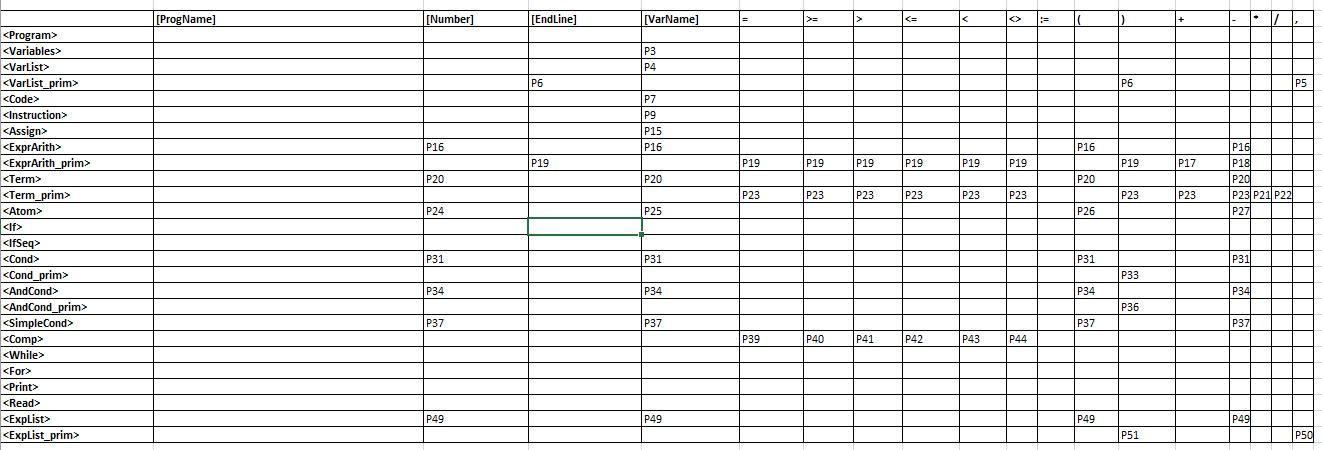
\includegraphics[height = 20 cm]{actionTable1.JPG}
    \caption{Action table 1}
    \label{fig:table1}
\end{figure}

\begin{figure}[!h]
    \centering
    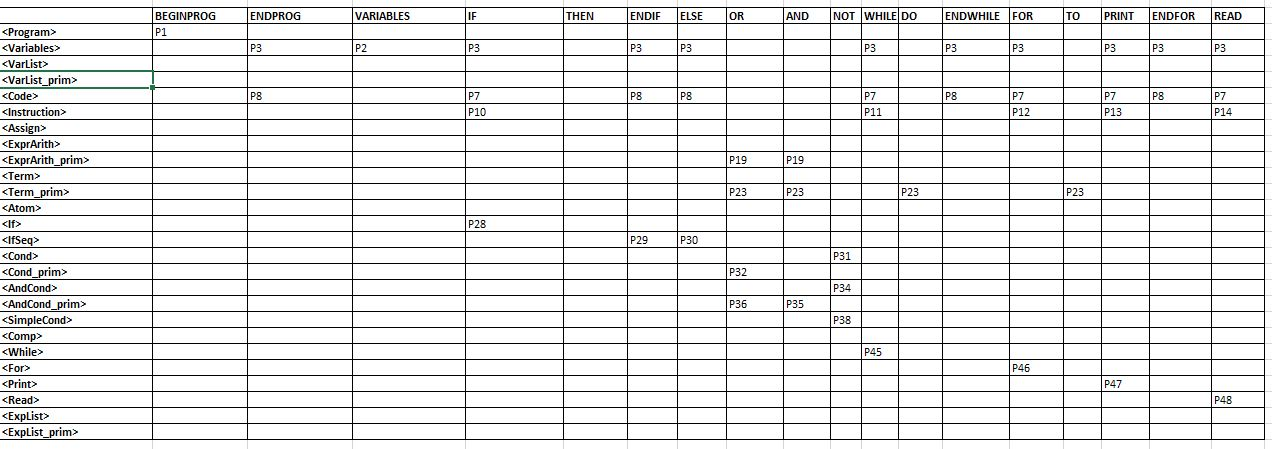
\includegraphics[height = 20 cm]{actionTable2.JPG}
    \caption{Action table 2}
    \label{fig:table2}
\end{figure}

\section {First and Follow}

\begin{figure}[H]
        \centering
        \includegraphics[width = 15cm] {firstANDFollow.JPG}
        \caption{First and Follow}
        \label{plot92}
\end{figure}


\section{Conclusion}

As we said in the introduction we implemented a LL(1) parser for the Super-Fortran programming language.

During this second part of the project we learned how to make a syntaxic analysis by
the building of a parser.
One major difficulty we faced was to transform the initial ambigous grammar to a none ambigous one
and to check if our transformation of the grammar was good.
A second difficulty was the verification of the firsts and follows because its easy to make mistakes
because the grammar had many produces and terminals.

But finally, this part of the project allowed us to learn more about the parsing step of a compiler 
and to understand deeply how it works.

\section{Annexe}
\end{document}
